\documentclass{article}

\usepackage{amsmath,amsfonts,amssymb,mathtools} % formatting math
\usepackage{amsthm} % for proofs
\usepackage{verbatim} % for block comments
\usepackage{hyperref} % for links

\hypersetup{
    colorlinks=true,
    linkcolor=blue,
    filecolor=magenta,      
    urlcolor=blue,
}

%+++++++++++++++++++++++++++++++

% FANCY LETTERS
\newcommand{\R}{\mathbb{R}} % the real number R
\newcommand{\E}{\mathbb{E}} % expectation symbol E

% BRACKETS, PARENTHESIS, AND CURLY BRACKETS
\newcommand{\lb}{\left[} % left bracket
\newcommand{\rb}{\right]} % right bracket
\newcommand{\lp}{\left(} % left parenthesis
\newcommand{\rp}{\right)} % right parenthesis
\newcommand{\lc}{\left\{} % left curly bracket
\newcommand{\rc}{\right\}} % right curly bracket

\title{Geometric Data Analysis HW 1}
\author{Gilad Turok, gt2453 \\ \href{mailto:gt2453@columbia.edu}{gt2453@columbia.edu}}
\date{\today}

\begin{document}
\maketitle

\section[]{$k$-means vs Single-Linkage Clustering}

    I generated data with three $2$-dimensional Gaussians with identity convariance matricies. I cluster this data with $k$-means and single-linkage clustering with means that vary. I use $4$ different sets of means, beginning from very close to each other to further and further apart:

    \begin{align*}
        \mu_1 = \begin{bmatrix} 0 \\ 0 \end{bmatrix}, \quad \mu_2 = \begin{bmatrix} 0 \\ 0 \\ \end{bmatrix}, \quad \mu_3 = \begin{bmatrix} 0 \\ 0 \end{bmatrix} \\
        \mu_1 = \begin{bmatrix} -2 \\ 2 \end{bmatrix}, \quad \mu_2 = \begin{bmatrix} 0 \\ -2 \end{bmatrix}, \quad \mu_3 = \begin{bmatrix} 2 \\ 2 \end{bmatrix} \\
        \mu_1 = \begin{bmatrix} -5 \\ 5 \end{bmatrix}, \quad \mu_2 = \begin{bmatrix} 0 \\ -5 \end{bmatrix}, \quad \mu_3 = \begin{bmatrix} 5 \\ 5 \end{bmatrix} \\
        \mu_1 = \begin{bmatrix} -10 \\ 10 \end{bmatrix}, \quad \mu_2 = \begin{bmatrix} 10 \\ -10 \end{bmatrix}, \quad \mu_3 = \begin{bmatrix} 10 \\ 10 \end{bmatrix} \\
    \end{align*}

    I noticed that the $k$-means algorithm is very sensitive to the initial means. If the initial means are too far apart, the algorithm will not converge. If the initial means are too close together, the algorithm will converge to a local minimum. The single-linkage clustering algorithm is not sensitive to the initial means. The single-linkage clustering algorithm will always converge to the same result, regardless of the initial means. The $k$-means algorithm will converge to different results depending on the initial means. The $k$-means algorithm will converge to the same result as the single-linkage clustering algorithm if the initial means are close enough to the true means. The $k$-means algorithm will converge to a different result than the single-linkage clustering algorithm if the initial means are too far apart from the true means.

    \begin{figure}[h]
        \label{fig:kmeans_singlelinkage}
        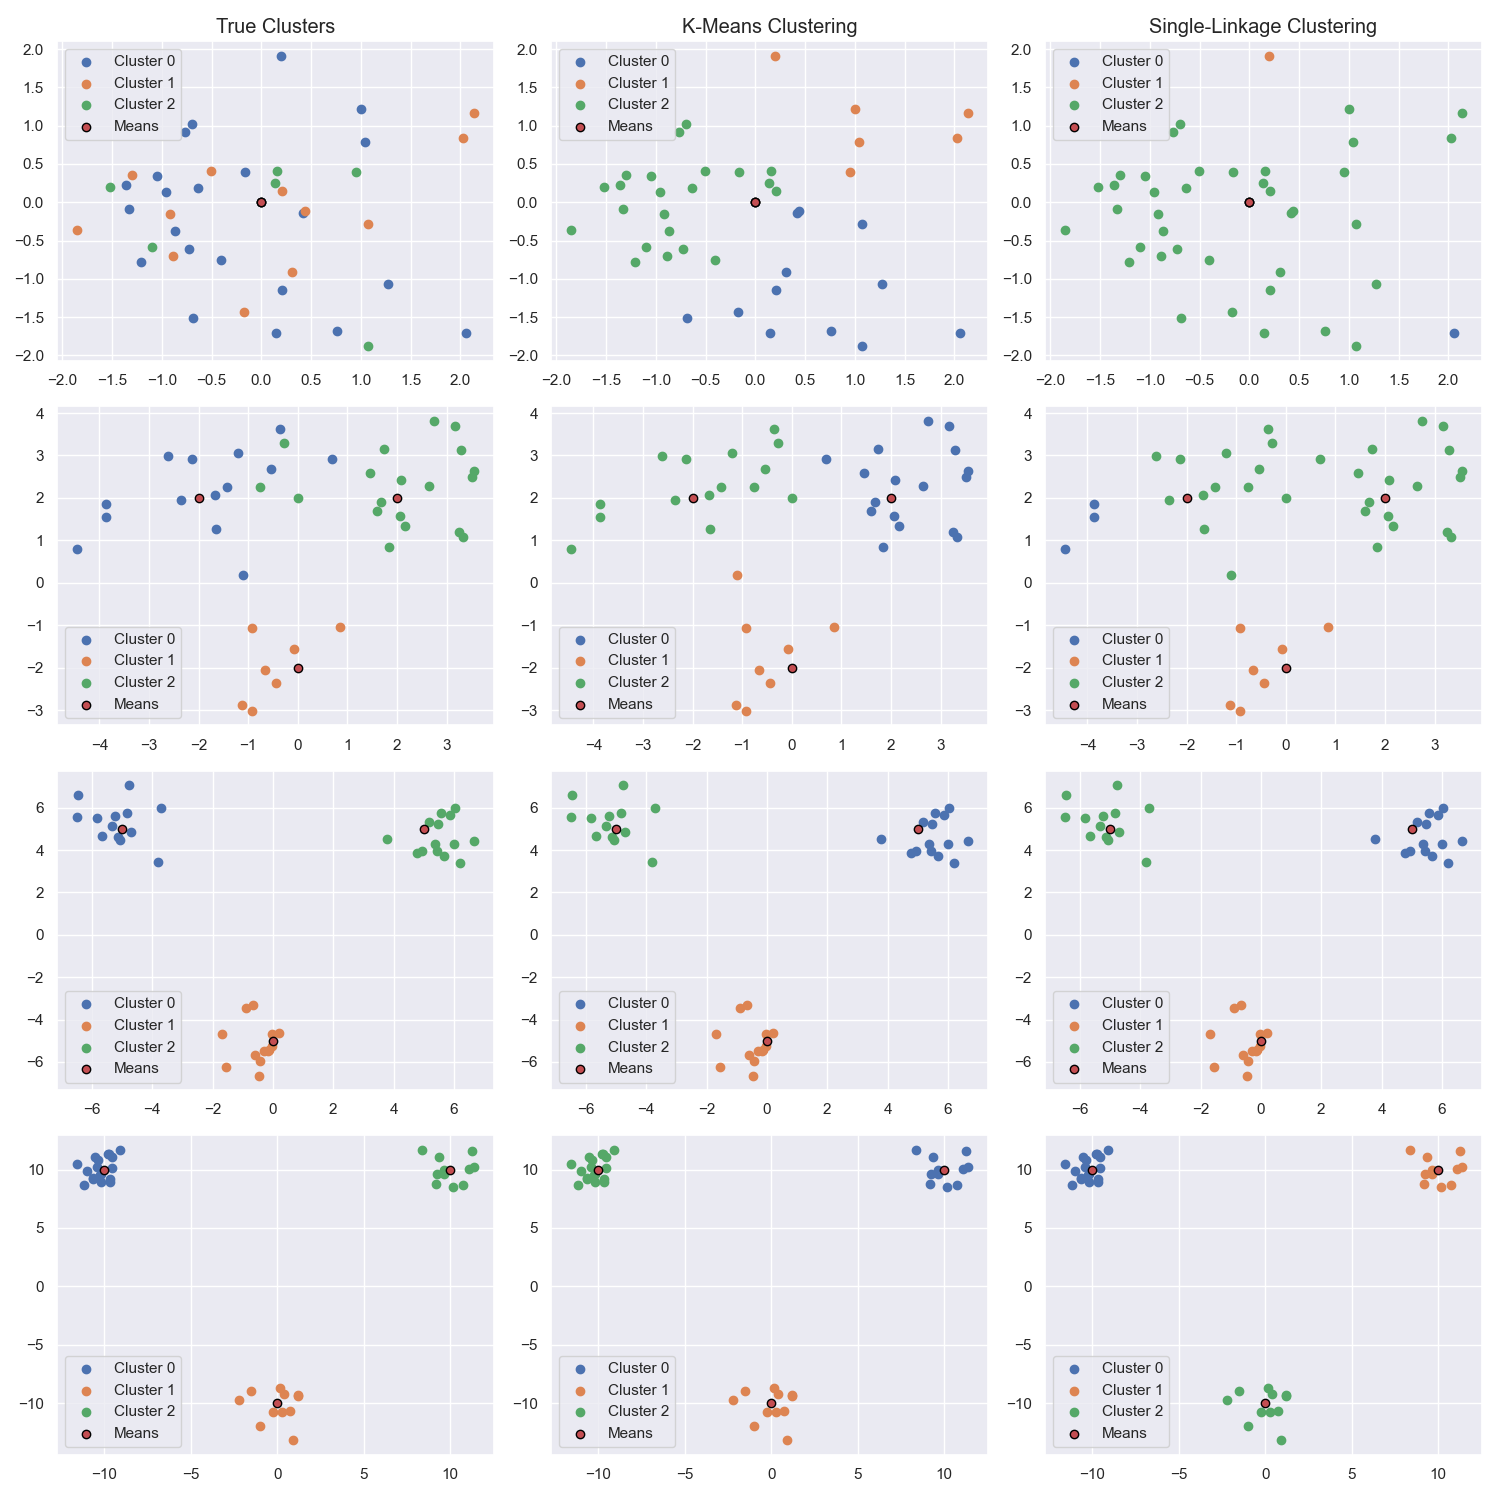
\includegraphics[width=0.99\linewidth]{images/q1/kmeans_singlelinkage.png}
        \caption{$k$-means vs single-linkage clustering on $3$ Gaussians with means at different distances}
    \end{figure}
    \pagebreak

\end{document}